% ERA-Großpraktikum: Entwickleranleitung -- Erweiterung

\section{Erweiterung}
Der folgende Abschnitt soll Anhaltspunkte zur Erweiterung des Simulators bieten. Eine Erweiterung kann entweder ein neues Assembler-Paket (also die Unterstützung einer neuen Assembler-Sprache, z.B. Intel-386\todo{Stimmt der Name?}) oder ein neues Modul (''Extension'') für das bereits vorhandene Assembler-Paket RISC-V (z.B. das Modul RV32F) sein. Des Weiteren ist es auch möglich, weitere Komponenten in der GUI zu ergänzen.\\

Da der Simulator für mehrere Assembler-Pakete konzipiert worden ist, müssen große Teile der Benutzeroberfläche und auch der Grundstruktur nicht neu geschrieben bzw. verändert werden. Vielmehr kommt es darauf an, das Konzept der bereits vorhandenen Teile zu verstehen und anzuwenden.

\subsection{Übersicht zur Architektur}
Um zu verstehen, wo die Erweiterung im Konzept einzuordnen ist, und welche Klassen zu implementieren sind, sollte man den Prozess verstehen, wie genau ein Assembler-Paket geladen und angesprochen wird. Einen groben Überblick bietet folgendes Diagramm. Die Namen der Komponenten finden sich so nicht im Code wieder, sie dienen lediglich als Oberbegriff für eine ganze Reihe von Klassen und -strukturen die grob die selbe Aufgabe haben.
\begin{figure}
	\centering
	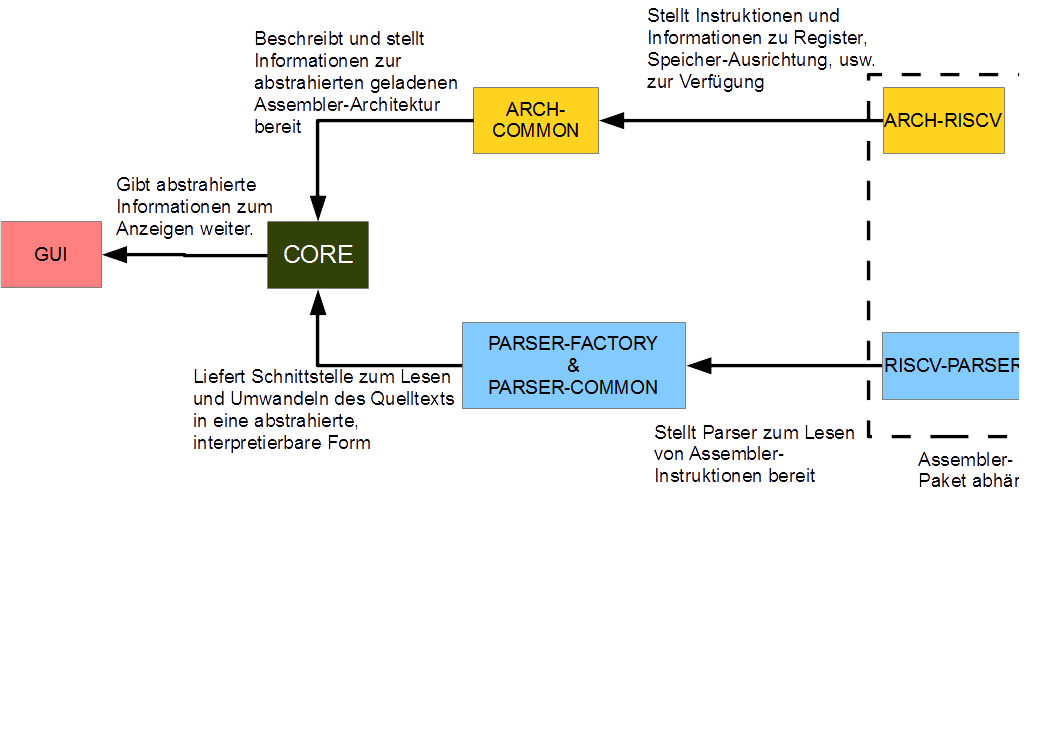
\includegraphics[scale=0.5]{charts/extension-overview.png}
	\label{dev-manual-extension-overview}
\end{figure}
\todo[inline]{Besseres Bild kommt noch (Erik)}
Nach der Auswahl des Assembler-Pakets durch den Benutzer in der Benutzeroberfläche werden ausgewählter Architekturname, gewählte Extensions und der gewählte Parser an den Core übergeben. Dieser lädt über Arch-Common Daten des Pakets und seinen Extensions, anschließend wird der passende Parser über die Parser-Factory erzeugt. Die Daten von Arch-Common enthalten zum Einen standardisierte, abstrahierte Informationen zum geladenen Paket (z.B. Länge, Anzahl, Funktion und Name von Registern, Speicher-Ausrichtung, Endianness, ...) und zum Anderen Zugriff auf Factories zur Erezugung von Instruktionsknoten.\\
Soll jetzt ein Quelltext eingelesen und ausgeführt werden, bekommt der Core den Text und gibt diesen an die geladene Parser-Implementierung weiter. Diese Implementierung wandelt das Programm in eine paket-unabhängige Darstellung mithilfe eines Syntaxbaumes um. Die Knoten des Syntaxbaums kann der Parser dabei über die Knoten-Factories der geladenen Architektur beziehen. Die paket-unabhängige Darstellung wird daraufhin vom Core ausgeführt. Alle Effekte auf Register und Speicher passieren in einer abstrahierten Art, so dass die Benutzeroberfläche Veränderungen anzeigen kann, ohne die konkrete Implementierung der Architektur zu kennen.\\

Es sind also nur diejenigen Teile zu implementieren, die im Diagramm gestrichelt umrandet sind. Es muss eine Architekturdefinition inklusive Implementierungen der einzelnen Instruktionen und ein Parser für diese geschrieben werden.

\subsection{Implementierung des Architektur-Teils}
Wie schon in \autoref{dev-manual-extension-overview} zu sehen, gibt es einen Teil, der bei jedem Paket existiert und die entsprechende Abstraktion nach außen (also Core und GUI) aufbaut. Der Architektur-Teil lässt sich weiter untergliedern in Definition und Eigenschaften des Assembler-Pakets, Bereitstellen der Instruktionen für den Parser zum Bau eines Syntaxbaumes und Implementierung des Verhaltens der Instruktionen.
\begin{figure}[ht]
	\centering
	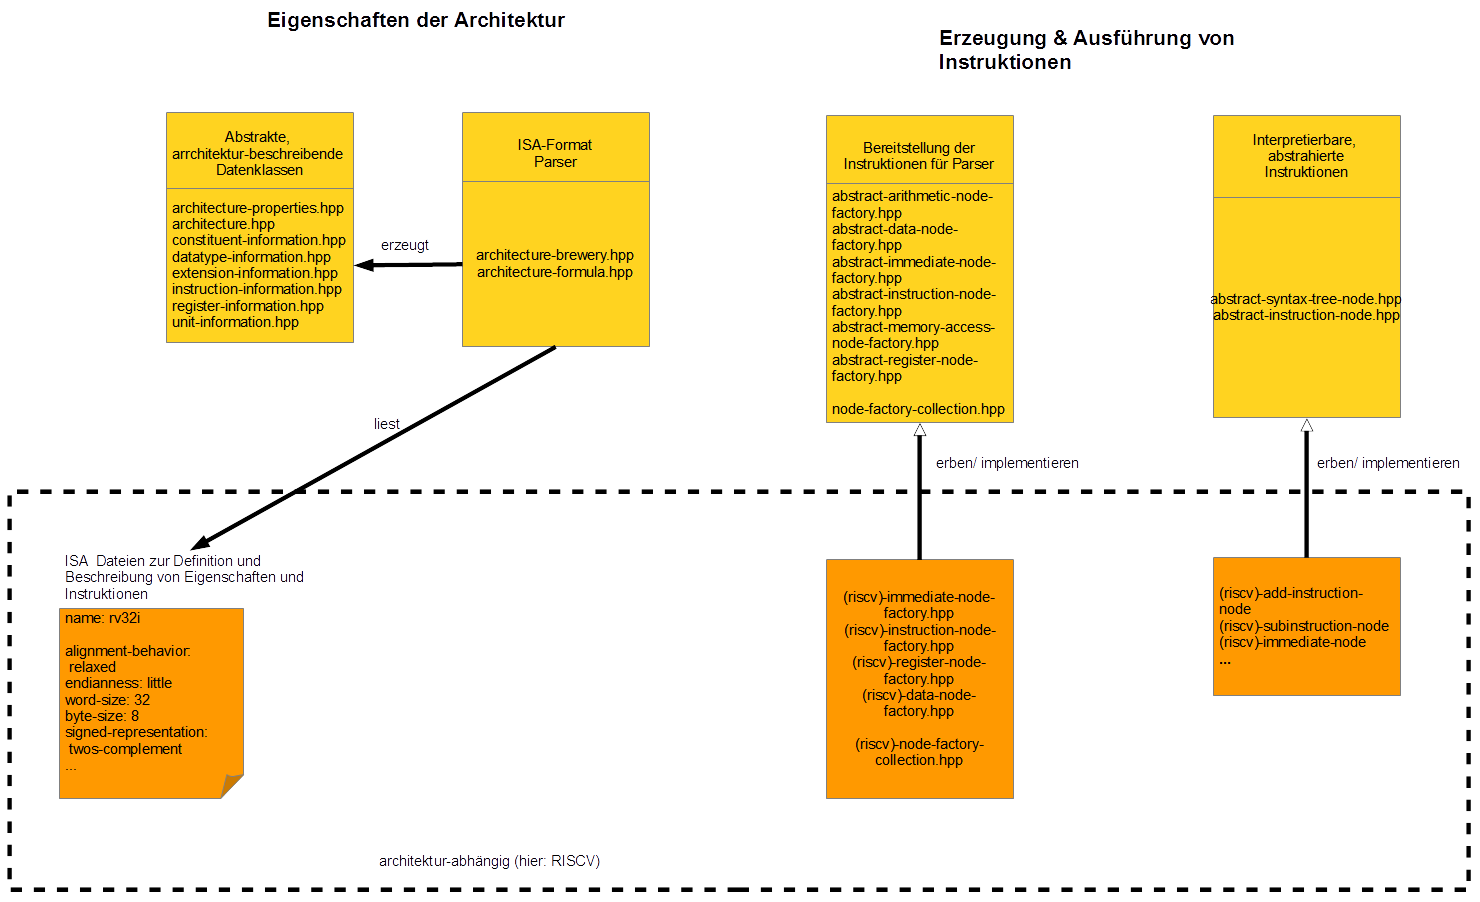
\includegraphics[scale=0.45]{charts/extension-arch.png}
\end{figure}

\subsubsection{Definition und Eigenschaften des Assembler-Pakets}
Für diesen Bereich ist keine Zeile Code nötig. Da eine Implementierung von Datenklassen zur Beschreibung der Eigenschaften sich inhaltlich, aber nicht strukturell unterscheiden wird, muss für eine Erweiterung lediglich eine Beschreibungsdatei im ISA-Format\todo{Verweis zur Beschreibung der ISA-Sprache} erstellt werden. Die Datei wird in YAML geschrieben, dann per Script nach JSON übersetzt und in den \texttt{isa} Ordner des Simulators abgelegt. Dort wird dann bei Programmstart und entsprechender Auswahl die JSON Datei eingelesen und bereits vorhandene Datenklassen mit Werten befüllt. Speicherort und Name der ISA-Dateien wird so erwartet: Innerhalb des ISA Ordners liegt ein Ordner mit Namen der Architektur. Innerhalb dieses Ordners liegen Ordner mit Namen der Extensions (auch die Basis bzw. Grundversion ist eine Extension), in denen wiederum befindet sich die JSON Datei \texttt{config.json} (und der Bequemlichkeit halber auch das YAML Gegenstück). Beispiel: Das Paket \texttt{xyz} hat ein Basismodul \texttt{xyz1}und eine Erweiterung \texttt{xyz2}:
\begin{lstlisting}
	era-gp-sim -- isa -- riscv.isa -- ...
	                  |- test.isa  -- ...
	                  |- xyz.isa   -- xyz1 -- config.json
	                               |       \- config.yaml
	                               \- xyz2 -- config.json
	                                       \- config.yaml
\end{lstlisting}
In den ISA-Files werden folgende Eigenschaften definiert:
\begin{itemize}
	\item Name, Wortgröße, Endiannes des Pakets
	\item Name, Größe, Funktion (Programmzähler, Flag, etc.) und Startwert der Register
	\item Name, Format der Assemblierung, Opcode jeder Instruktion
	\item (Optional) Definition von Makros (sofern Makros vom Parser unterstützt werden), die der Benutzer verwenden kann
\end{itemize}

\subsubsection{Bereitstellen der Instruktionen für den Parser}
\label{extension-arch-factories}
Der Parser baut beim Übersetzen aus jedem Befehl einen Syntaxbaum. Die Knoten dieses Baumes erhalten dann durch Polymorphie ihr architektur-spezifisches Verhalten (siehe \autoref{extension-arch-ast}). Der Parser kennt aber die genauen Signaturen und damit die Implementierungen der Syntaxbaumknoten nicht. Um zur Laufzeit trotzdem die richtige Knotenimplementierung zu erzeugen, verwenden wir hier das Factory-Design-Pattern\footnote{https://de.wikipedia.org/wiki/Fabrikmethode}. Folgende (abstrakte) Knoten-Fabriken sollten implementiert werden. Wird eine Fabrik nicht implementiert (z.B. bei RISC-V \texttt{arithmetic-node-factory}) ist das in Ordnung, solange der Parser die Fabrik nicht verwendet. Da aber sowohl Parser als auch Fabrik-Implementierung in einer Erweiterung entstehen müssen, sollte das kein Problem darstellen. Jede Fabrik-Klasse erzeugt genau eine Art von Knoten (\autoref{} \todo{Verweis zu 3.3.1}):
\begin{itemize}
	\item \textbf{Arithmetic-Node Factory}: Erzeugt Knoten für arithmetische Operationen. Da diese Knotenart in RISC-V nicht genutzt wird, ist die Fabrik lediglich spezifiziert, aber nicht implementiert.
	
	\item \textbf{Data-Node-Factory}: Erzeugt Knoten, die binäre Daten verwalten. In RISC-V halten diese Knoten String-Literale (zur Verwendung in \texttt{simucrash}).
	
	\item \textbf{Immediate-Node-Factory}: Erzeugt Knoten, die Konstanten verwalten. 
	
	\item \textbf{Instruction-Node-Factory}: Erzeugt Knoten für die jeweiligen Instruktionen. Im Gegensatz zu den anderen Fabriken müssen hier (je nach Architektur) sehr viele verschiedene Implementierungen zurückgegeben werden.
	
	\item \textbf{Memory-Access-Node-Factory}: Erzeugt Knoten, die einen Speicherzugriff zur Laufzeit machen. Da diese Knotenart in RISC-V nicht genutzt wird, ist die Fabrik lediglich spezifiziert, aber nicht implementiert.
	
	\item \textbf{Register-Node-Factory}: Erzeugt Knoten, die auf ein Register zugreifen.
\end{itemize}
Da das Verwalten von bis zu sechs Fabriken für eine Parserimplementierung unübersichtlich wird, gibt es einzige Instanz (\texttt{NodeFactoryCollection}) die das Interface der einzelnen Fabriken spiegelt und Aufrufe entsprechend weiterleitet. Die Parserimplementierung muss nur die \texttt{NodeFactoryCollection}-Instanz verwalten.\\
Die NodeFactoryCollection wird automatisch beim Laden der Architektur aus den ISA-Dateien erzeugt und dem Architektur-Objekt als Member mitgegeben. Damit das funktioniert muss in \texttt{arch/commons/node-factory-collection-maker.cpp} in der Funktion \texttt{CreateFor} für die neue Architektur eine passende NodeFactoryCollection zurückgegeben werden.\\
Für RISC-V haben wir im riscv-namespace eine NodeFactoryCollection mit den RISC-V Implementierungen der benötigten Fabriken definiert (siehe \texttt{arch/riscv/factory-types.hpp}).

\subsubsection{Implementierung der Instruktionen}
\label{extension-arch-ast}
Der zentrale und auch für den Nutzer sichtbare Teil einer neuen Architektur sind die neuen Instruktionen. Eine konkrete Instruktion also z.B. \texttt{addi x1, x0, 0x45 (riscv)} wird intern als Syntaxbaum dargestellt. Der Parser verwandelt jede Zeile Quelltext in einen Baum. Diese Liste an Bäumen repräsentiert dann das ausführbare Programm. Da der Parser nur die syntaktische Bedeutung eines Symbols kennt, nicht aber seine Semantik (also das Verhalten, die Implementierung), ruft der Parser die passende Fabrik auf, die dann eine semantisch passende Implementierung instanziiert und zurückgibt. Der Parser kann aufgrund z.B. der Position des Symbols auf seine syntaktische Rolle schließen. Das erste Word, das keine Direktive oder Marke ist, muss der mnemotechnische Befehl sein; der Ausdruck danach muss der erste Operand sein, usw. Die Implementierung der Fabriken wurde in \autoref{extension-arch-factories} bereits behandelt. 

\subsection{Erweiterung der GUI}
Soll eine neue Komponente zur GUI hinzugefügt werden, gibt es mehrere Entscheidungen zu treffen. Die Komponente kann etwas bestehendes, wie die Ausgabe, erweitern oder komplett neu sein. in diesem Fall gilt es noch zu klären, ob sie Projektspezifisch, wie Speicher oder Register, ist oder auf das ganze Programm, also außerhalb der TabView wie die Menubar, bezogen werden soll.

\subsubsection{Erweiterung bestehender Komponenten}
Das Erweitern bestehender Komponenten ist vergleichsweise einfach. Hier gilt es, in der entsprechenden C++-Datei nachzuschlagen. Ist, wie bei der Ausgabe, nur eine für die gesamte Komponente angelegt, müssen hier etwaige Attribute und Methoden ergänzt werden. Ist dagegen für jeden einzelnen Teil eine eigene Datei angelegt, so sollte auch für die Erweiterung eine ergänzt werden. Man beachte, dass es wahrscheinlich nötig sein wird, die Instanzen zum \texttt{QQMLContext} hinzuzufügen.\\
In QML sind Komponenten, die mehrere eigene Module besitzen, üblicherweise in einer TabView dargestellt. Es muss also nur ein Tab in der Hauptdatei der zu erweiternden Komponente ergänzt werden. Die eigentliche Definition sollte in einer eigenen Datei in einem neuen Unterverzeichnis erfolgen. Im Allgemeinen sollte auch auf ein Einstellungsfenster, die entsprechende Funktion und die Themes geachtet werden. Um zu erkennen, ob dies nötig ist, beachte man die anderen Module.

\subsubsection{Neue Komponenten}
Auch das Hinzufügen neuer Komponenten gestaltet sich nicht besonders schwierig. Für den QML-Teil ist Folgendes zu tun: Im Ordner \texttt{ui/Components} ein neuer Ordner angelegt werden. Dort werden alle neuen Dateien der Erweiterung abgelegt. Außerhalb dieses Ordners muss nur die Datei \texttt{ui/SplitviewItem.qml} modifiziert werden. Hier muss in der ComboBox der entsprechende Name eingetragen werden, in den Variablen \texttt{model} und \texttt{usualList}. Außerdem muss unten im Loader der Pfad der Hauptdatei hinzugefügt werden, am gleichen Index wie der Name in der ComboBox. Des weiteren sei bemerkt, dass jede neue Komponente eine Variable \texttt{hasComponentSettings} benötigt.\\
 Der C++-Teil wird einfach unter \texttt{ui} abgelegt. Auch ein Header sollte im entsprechenden Verzeichnis vorhanden sein. Soll die Komponente für jedes Projekt einzeln verwendet werden, so wird eine neue Instanz der C++-Klasse in der entsprechenden Instanz der Klasse \texttt{GuiProject} hinterlegt. Von dort kann man auch den \texttt{QQmlContext} bekommen. Dieser ist zwingend nötig, wenn aus QML auf die C++ Instanz zugegriffen werden soll. Ist die neue Komponente dagegen für alle Projekte gleich, so verwende man die \texttt{Ui} Klasse. Bei der Programmierung der neuen C++-Klasse sollte der Abschnitt zur Kommunikation der Module beachtet werden, siehe \autoref{gui-kommunikation}.
 



